\documentclass[border=10pt]{standalone}
\usepackage{tikz}
\usepackage{xcolor}

% Couleurs
\definecolor{containercolor}{RGB}{102,102,115}
\definecolor{watercolor}{RGB}{51,153,255}
\definecolor{precontainercolor}{RGB}{255,128,0}
\definecolor{postcontainercolor}{RGB}{128,0,128}
\definecolor{aircolor}{RGB}{220,240,255}

\begin{document}
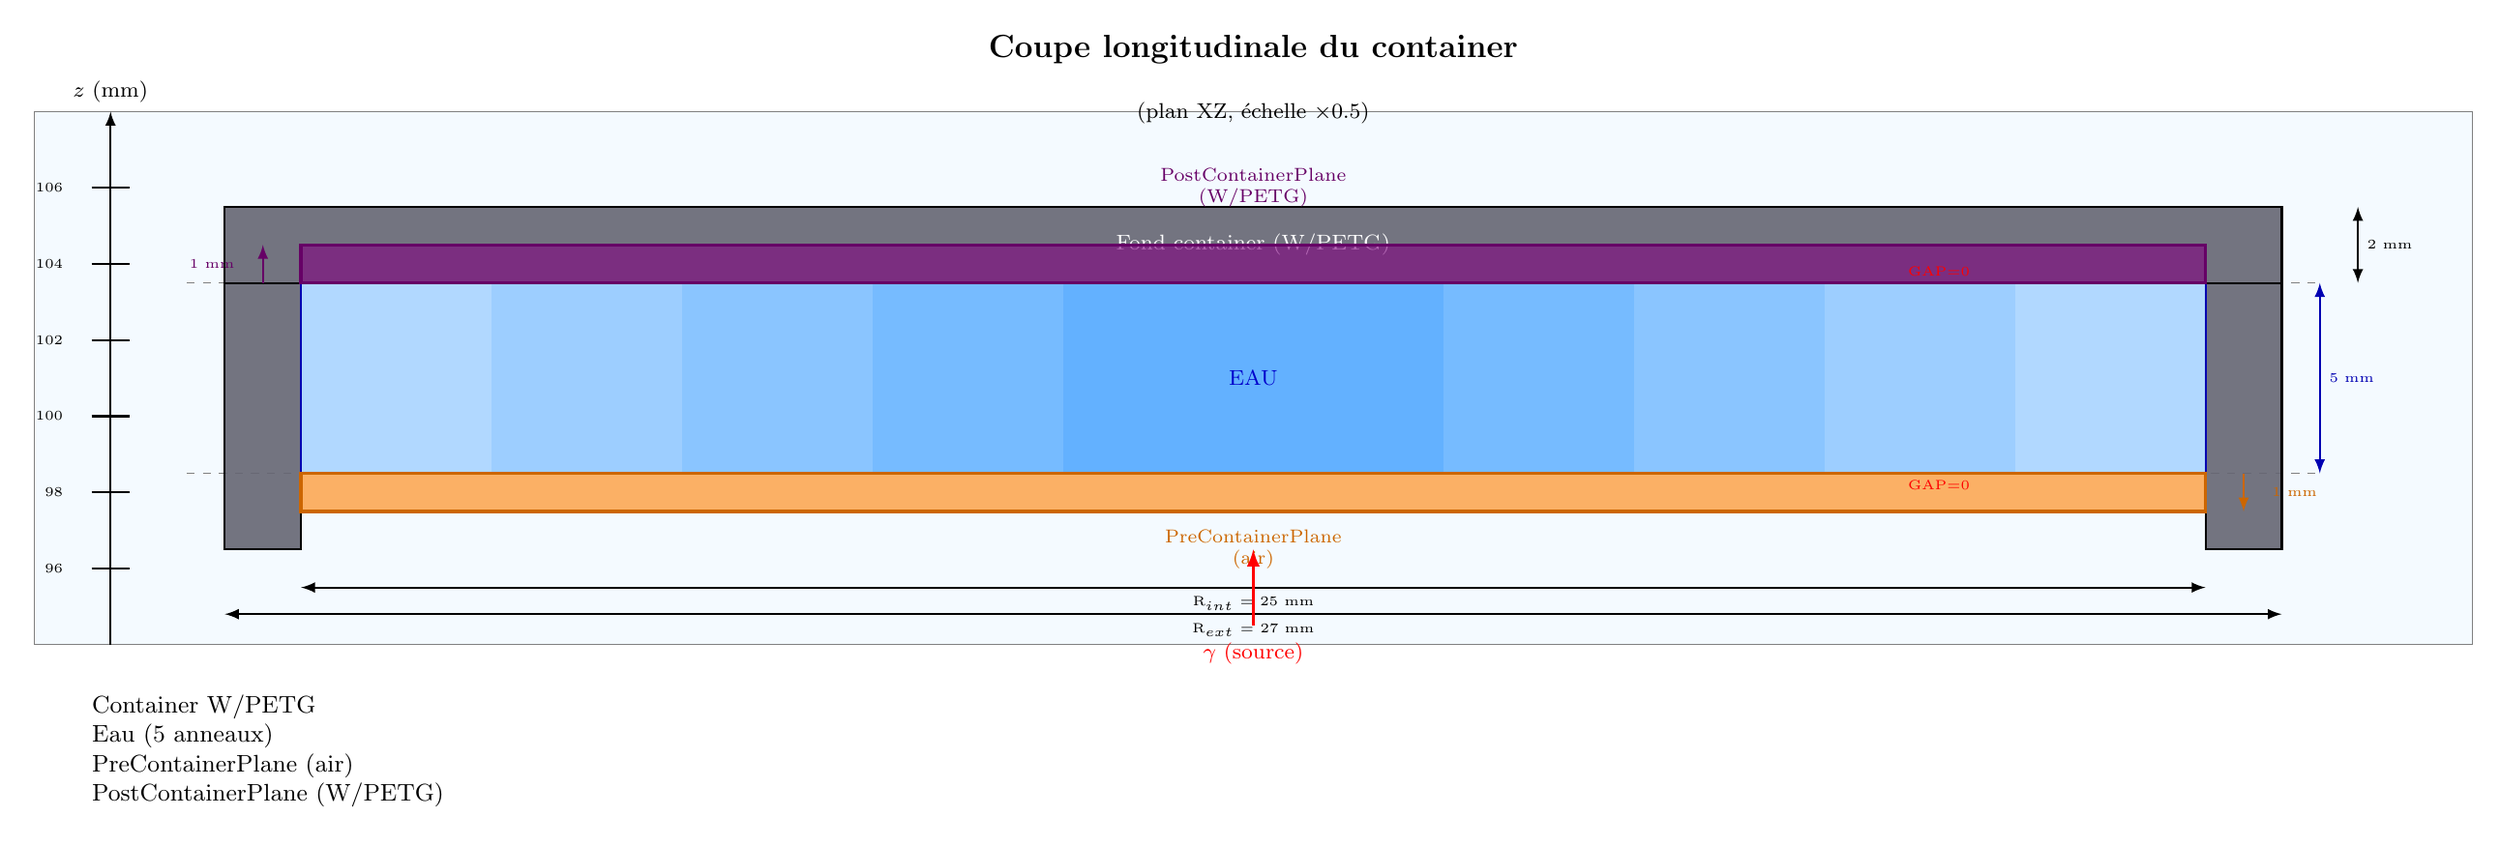
\begin{tikzpicture}[scale=0.5, >=latex]
    
    % ═══════════════════════════════════════════════════════════════
    % ÉCHELLE : 1 unité = 1 mm (échelle x0.5)
    % Vue en coupe longitudinale (plan XZ) - Container uniquement
    % Agrandissement : z de 94 mm à 108 mm, x de -32 mm à 32 mm
    % ═══════════════════════════════════════════════════════════════
    
    % Cadre et fond (air)
    \fill[aircolor, opacity=0.3] (-32,94) rectangle (32,108);
    \draw[gray, thin] (-32,94) rectangle (32,108);
    
    % ═══════════════════════════════════════════════════════════════
    % AXE DES Z (vertical) avec graduations
    % ═══════════════════════════════════════════════════════════════
    \draw[->, thick] (-30,94) -- (-30,108);
    \node[above, font=\footnotesize] at (-30,108) {$z$ (mm)};
    
    \foreach \z in {96,98,100,102,104,106} {
        \draw[thick] (-30.5,\z) -- (-29.5,\z);
        \node[left, font=\tiny] at (-31,\z) {\z};
    }
    
    % Lignes de référence horizontales (pointillées)
    \foreach \z in {98.5, 103.5} {
        \draw[gray, dashed, thin] (-28,\z) -- (28,\z);
    }
    
    % ═══════════════════════════════════════════════════════════════
    % CONTAINER - Parois latérales (W/PETG)
    % Rayon intérieur = 25 mm, extérieur = 27 mm
    % z de 96.5 à 103.5 mm (ouvert en bas, fermé en haut)
    % ═══════════════════════════════════════════════════════════════
    
    % Paroi gauche
    \fill[containercolor, opacity=0.9] (-27,96.5) rectangle (-25,103.5);
    \draw[black, thick] (-27,96.5) rectangle (-25,103.5);
    
    % Paroi droite
    \fill[containercolor, opacity=0.9] (25,96.5) rectangle (27,103.5);
    \draw[black, thick] (25,96.5) rectangle (27,103.5);
    
    % ═══════════════════════════════════════════════════════════════
    % CONTAINER - Fond (W/PETG)
    % z de 103.5 à 105.5 mm, rayon = 27 mm
    % ═══════════════════════════════════════════════════════════════
    
    \fill[containercolor, opacity=0.9] (-27,103.5) rectangle (27,105.5);
    \draw[black, thick] (-27,103.5) rectangle (27,105.5);
    \node[font=\footnotesize, white] at (0,104.5) {Fond container (W/PETG)};
    
    % ═══════════════════════════════════════════════════════════════
    % EAU - 5 anneaux concentriques (en coupe)
    % z de 98.5 à 103.5 mm (5 mm épaisseur)
    % Anneaux de 5 mm de largeur chacun
    % ═══════════════════════════════════════════════════════════════
    
    % Anneau 4 (externe) : r = 20-25 mm
    \fill[watercolor, opacity=0.35] (-25,98.5) rectangle (-20,103.5);
    \fill[watercolor, opacity=0.35] (20,98.5) rectangle (25,103.5);
    
    % Anneau 3 : r = 15-20 mm
    \fill[watercolor, opacity=0.45] (-20,98.5) rectangle (-15,103.5);
    \fill[watercolor, opacity=0.45] (15,98.5) rectangle (20,103.5);
    
    % Anneau 2 : r = 10-15 mm
    \fill[watercolor, opacity=0.55] (-15,98.5) rectangle (-10,103.5);
    \fill[watercolor, opacity=0.55] (10,98.5) rectangle (15,103.5);
    
    % Anneau 1 : r = 5-10 mm
    \fill[watercolor, opacity=0.65] (-10,98.5) rectangle (-5,103.5);
    \fill[watercolor, opacity=0.65] (5,98.5) rectangle (10,103.5);
    
    % Anneau 0 (central) : r = 0-5 mm
    \fill[watercolor, opacity=0.75] (-5,98.5) rectangle (5,103.5);
    
    % Contour eau
    \draw[blue!70!black, thick] (-25,98.5) rectangle (25,103.5);
    \node[font=\footnotesize, blue!80!black] at (0,101) {EAU};
    
    % ═══════════════════════════════════════════════════════════════
    % PLAN PRE-CONTAINER (Orange, Air)
    % z centre = 98.0 mm, épaisseur = 1 mm
    % Limite haute = 98.5 mm (bas de l'eau) - GAP=0
    % ═══════════════════════════════════════════════════════════════
    
    \fill[precontainercolor, opacity=0.6] (-25,97.5) rectangle (25,98.5);
    \draw[precontainercolor!80!black, very thick] (-25,97.5) rectangle (25,98.5);
    \node[font=\scriptsize, precontainercolor!80!black, align=center] at (0,96.5) 
        {PreContainerPlane\\(air)};
    
    % Flèche indiquant la limite
    \draw[precontainercolor!80!black, thick, ->] (26,98.5) -- (26,97.5);
    \node[right, font=\tiny, precontainercolor!80!black] at (26.5,98) {1 mm};
    
    % ═══════════════════════════════════════════════════════════════
    % PLAN POST-CONTAINER (Violet, W/PETG)
    % z centre = 104.0 mm, épaisseur = 1 mm
    % Limite basse = 103.5 mm (haut de l'eau) - GAP=0
    % ═══════════════════════════════════════════════════════════════
    
    \fill[postcontainercolor, opacity=0.6] (-25,103.5) rectangle (25,104.5);
    \draw[postcontainercolor!80!black, very thick] (-25,103.5) rectangle (25,104.5);
    \node[font=\scriptsize, postcontainercolor!80!black, align=center] at (0,106) 
        {PostContainerPlane\\(W/PETG)};
    
    % Flèche indiquant la limite
    \draw[postcontainercolor!80!black, thick, ->] (-26,103.5) -- (-26,104.5);
    \node[left, font=\tiny, postcontainercolor!80!black] at (-26.5,104) {1 mm};
    
    % ═══════════════════════════════════════════════════════════════
    % COTES ET ANNOTATIONS
    % ═══════════════════════════════════════════════════════════════
    
    % Cote épaisseur eau
    \draw[<->, blue!70!black, thick] (28,98.5) -- (28,103.5);
    \node[right, font=\tiny, blue!70!black] at (28,101) {5 mm};
    
    % Cote épaisseur fond container
    \draw[<->, black, thick] (29,103.5) -- (29,105.5);
    \node[right, font=\tiny] at (29,104.5) {2 mm};
    
    % Cote rayon eau/container
    \draw[<->, thick] (-25,95.5) -- (25,95.5);
    \node[below, font=\tiny] at (0,95.5) {R$_{\text{int}}$ = 25 mm};
    
    % Cote rayon externe
    \draw[<->, thick] (-27,94.8) -- (27,94.8);
    \node[below, font=\tiny] at (0,94.8) {R$_{\text{ext}}$ = 27 mm};
    
    % Annotation GAP=0
    \node[font=\tiny, red] at (18,98.2) {GAP=0};
    \node[font=\tiny, red] at (18,103.8) {GAP=0};
    
    % ═══════════════════════════════════════════════════════════════
    % FLÈCHE DIRECTION SOURCE (bas)
    % ═══════════════════════════════════════════════════════════════
    
    \draw[->, red, very thick] (0,94.5) -- (0,96.5);
    \node[below, font=\footnotesize, red] at (0,94.3) {$\gamma$ (source)};
    
    % ═══════════════════════════════════════════════════════════════
    % LÉGENDE
    % ═══════════════════════════════════════════════════════════════
    
    \node[font=\small, anchor=north west] at (-32,93) {
        \begin{tabular}{ll}
            \textcolor{containercolor}{$\blacksquare$} & Container W/PETG \\
            \textcolor{watercolor}{$\blacksquare$} & Eau (5 anneaux) \\
            \textcolor{precontainercolor}{$\blacksquare$} & PreContainerPlane (air) \\
            \textcolor{postcontainercolor}{$\blacksquare$} & PostContainerPlane (W/PETG) \\
        \end{tabular}
    };
    
    % ═══════════════════════════════════════════════════════════════
    % TITRE
    % ═══════════════════════════════════════════════════════════════
    
    \node[font=\large\bfseries, anchor=south] at (0,109) {Coupe longitudinale du container};
    \node[font=\footnotesize, anchor=north] at (0,108.5) {(plan XZ, échelle $\times$0.5)};
    
\end{tikzpicture}
\end{document}
